\documentclass[12pt]{article}
% \usepackage{fullpage}
% \usepackage{enumitem}
\usepackage{amsmath,amssymb,graphicx}
% \usepackage{booktabs}
\usepackage{amsmath,amssymb,graphicx}

% \usepackage{sectsty}
% \usepackage{float}
% \usepackage{parskip}
\sectionfont{\fontsize{15}{20}\selectfont}


\DeclareMathOperator*{\argmax}{arg\,max}
\DeclareMathOperator*{\argmin}{arg\,min}
\DeclareMathOperator{\E}{\mathbb{E}}
\newcommand{\dataset}{\mathcal{D}}
\newcommand{\task}{\mathcal{T}}
\newcommand{\supportdata}{\mathcal{D}^\mathrm{tr}}
\newcommand{\querydata}{\mathcal{D}^\mathrm{ts}}
\newcommand{\support}[1]{{#1}^\mathrm{tr}}
\newcommand{\query}[1]{{#1}^\mathrm{ts}}
% \usepackage{bbm}
% \usepackage{gensymb}
% \usepackage{xcolor}
\usepackage{color}

% \usepackage{tgpagella}

\begin{document}

\begin{center}
{{\Large \textbf{CS 330 Autumn 2022 Homework 3 \\ Goal Conditioned Reinforcement Learning and Hindsight Experience Replay}}
\\ {\large Due Wednesday October 27th, 11:59 PM PT}}

\begin{tabular}{rl}
SUNet ID: &  \\
Name: & \\
Collaborators: & 
\end{tabular}
\end{center}

By turning in this assignment, I agree by the Stanford honor code and declare that all of this is my own work.

\newpage
\section*{Problem 3: Analyzing HER for Bit Flipping Environment}

\subsubsection*{a) num bits=6}

\begin{figure}[h!]
\centering
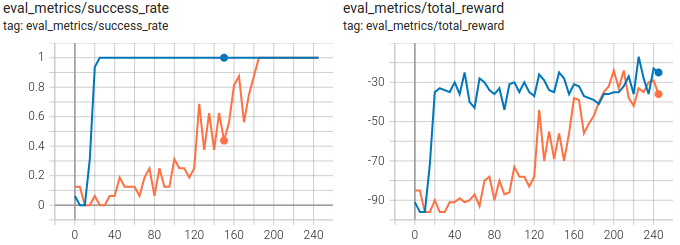
\includegraphics[width=1.0\linewidth]{figures/q3-a}
\vspace{-3mm}
\caption{Orange: No HER, Blue: HER-Final}
\label{fig:q3a}
\end{figure}


\subsubsection*{b) num bits=15}

\begin{figure}[h!]
\centering
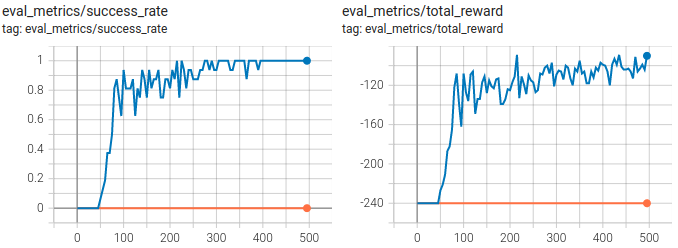
\includegraphics[width=1.0\linewidth]{figures/q3-b}
\vspace{-3mm}
\caption{Orange: No HER, Blue: HER-Final}
\label{fig:q3b}
\end{figure}

\newpage
\subsubsection*{c) num bits=25}

\begin{figure}[h!]
\centering
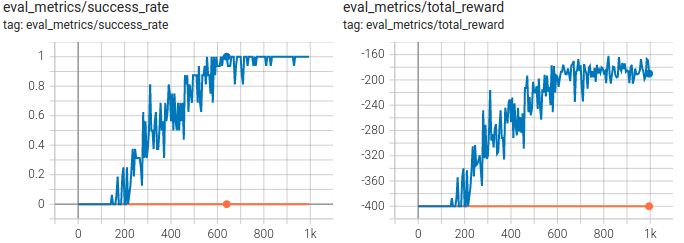
\includegraphics[width=1.0\linewidth]{figures/q3-c}
\vspace{-3mm}
\caption{Orange: No HER, Blue: HER-Final}
\label{fig:q3c}
\end{figure}


\subsubsection*{d) compare the three versions of HER for num bits=15}

\begin{figure}[h!]
\centering
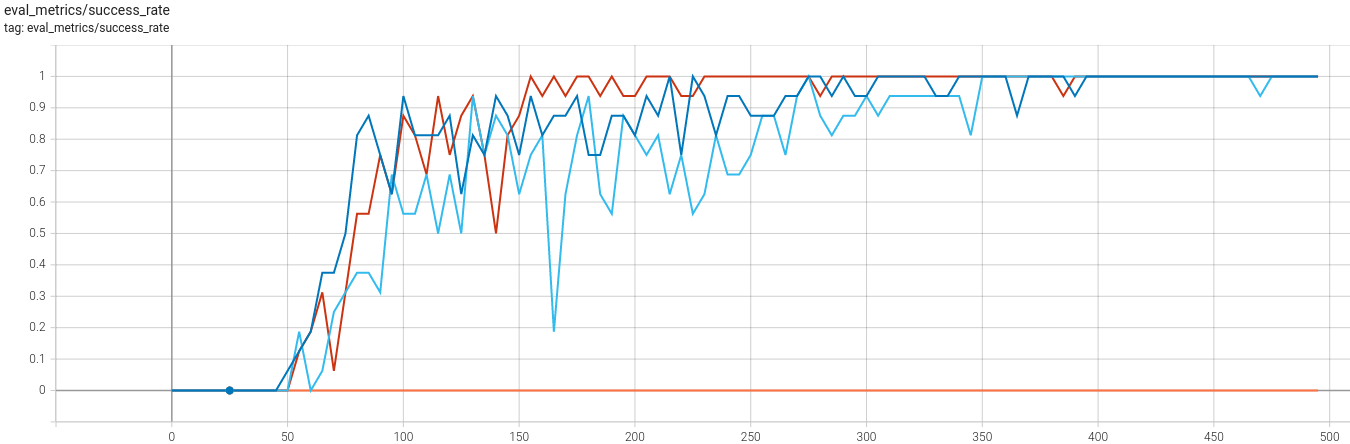
\includegraphics[width=1.0\linewidth]{figures/q3-d-1}
\vspace{-3mm}
\caption{Success Rate : Orange: No HER, Blue: HER-Final, Red: HER-Random, Turquoise: HER-Future }
\label{fig:q3d1}
\end{figure}

\begin{figure}[h!]
\centering
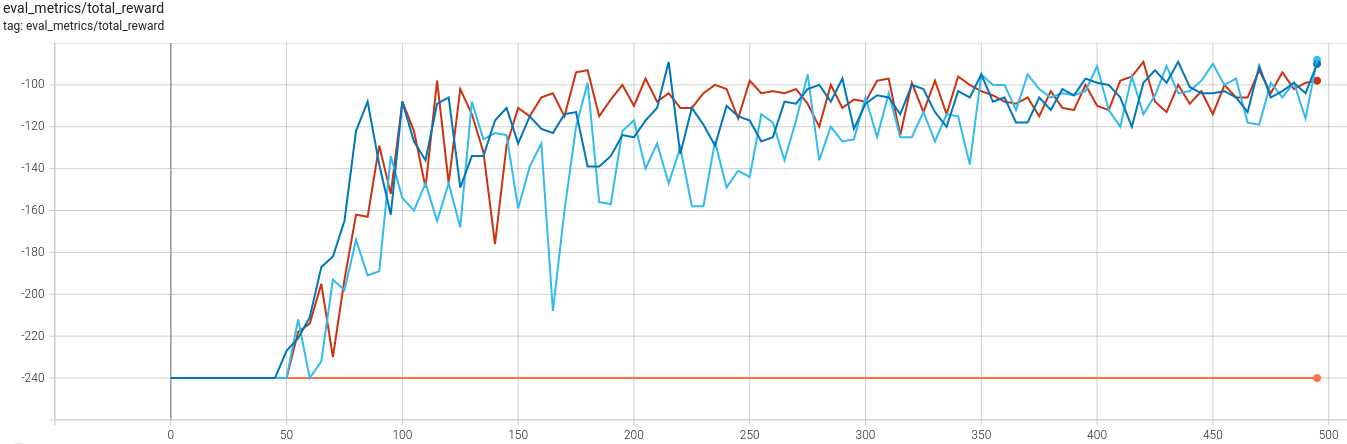
\includegraphics[width=1.0\linewidth]{figures/q3-d-2}
\vspace{-3mm}
\caption{Total Reward : Orange: No HER, Blue: HER-Final, Red: HER-Random, Turquoise: HER-Future }
\label{fig:q3d2}
\end{figure}

\newpage
\subsubsection*{e) Summary}

Using HER always improves performance. Without HER, success rate improves only for 6 bits.

HER-Final and HER-Random performs similarly. HER-Future performs slighly worse.

\newpage
\section*{Problem 4: Analyzing HER for Sawyer Reach}


\subsubsection*{a) Screenshots}

\begin{figure}[h!]
\centering
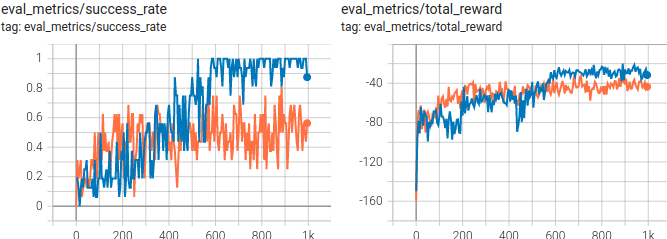
\includegraphics[width=1.0\linewidth]{figures/q4-a}
\vspace{-3mm}
\caption{Total Reward : Orange: No HER, Blue: HER-Final }
\label{fig:q4a}
\end{figure}

\subsubsection*{b) Summary}

    Success rate 1.0 is only achieved when HER is used.

\end{document}

